Η ενσωμάτωση του μοντέλου ελαστικών σε έναν προσομοιωτή γύρου απαιτεί τον ορισμό 
ενός μοντέλου οχήματος που να συνδέει τα κινηματικά μεγέθη (ταχύτητα, επιτάχυνση)
με τις δυνάμεις που αναπτύσσονται σε κάθε τροχό. Στην παρούσα εργασία χρησιμοποιείται
ένα \emph{δίτροχο μοντέλο} (two-track model) τριών βαθμών ελευθερίας: διαμήκης
ταχύτητα, πλευρική ταχύτητα και ρυθμό εκτροπής (yaw rate) $U_x,U_y,\dot{\psi} $. Το μοντέλο αντιμετωπίζει το 
σώμα ως άκαμπτο σώμα (rigid body) χωρίς δυναμική ανάρτησης. Η μοντελοποίηση του αμαξώματος
ως άκαμπτο είναι επαρκής: Η συμπερίληψη ενός ελαστικού
μοντέλου ανάρτησης θα βελτίωνε μεν την ακρίβεια του μοντέλου σε δυναμικές συνθήκες,
ωστόσο δεν παρέχει ουσιαστική βελτίωση στη φύση των αποτελεσμάτων που εξετάζει η παρούσα διπλωματική.

Η επιλογή δίτροχου έναντι μονότροχου (bicycle model) μοντέλου είναι εδώ αναγκαία: στο δίτροχο διακρίνονται
οι αριστεροί από τους δεξιούς τροχούς, γεγονός απαραίτητο για τον ανεξάρτητο υπολογισμό της θερμοκρασίας
κάθε τροχού.

% ---

\subsection{Συστήματα συντεταγμένων}
\label{subsec:frames}
% ---

Για τη μαθηματική περιγραφή της κίνησης χρησιμοποιούνται τρία ορθοκανονικά συστήματα συντεταγμένων,
τα οποία ορίζονται σύμφωνα με τις συμβάσεις SAE \cite{Milliken1995} -- ο άξονας $x$ βρίσκεται στη διαμήκη
διεύθυνση με κατεύθυνση την κατεύθυνση κίνησης, ο άξονας $y$ κατευθύνεται στην πλευρική διεύθυνση προς τα
αριστερά, και ο άξονας $z$ κατακόρυφα προς τα επάνω. Το κέντρο του συστήματος αξόνων λαμβάνεται στο κέντρο
μάζας του οχήματος\\[6pt]
\noindent Με βάση τη μοντελοποίηση του δίτροχου μοντέλου 3 βαθμών ελευθερίας, ορίζονται τα εξής συστήματα αξόνων.
\begin{itemize}
  \item Σύστημα $\hat{X}\hat{Y}\hat{Z}$ με τον άξονα $\hat{X}$ προσανατολισμένο με την τροχιά της πίστας.
  \item Τοπικό σύστημα οχήματος $xyz$, με τον άξονα $x$ τον διαμήκη του οχήματος.
  \item Τοπικό σύστημα τροχού $uvw$ -- ο άξονας $u$ είναι προσανατολισμένος με την κατεύθυνση κύλισης (ένα σύστημα για κάθε τροχό).
\end{itemize}

\begin{figure}[ht!]
    \begin{center}
        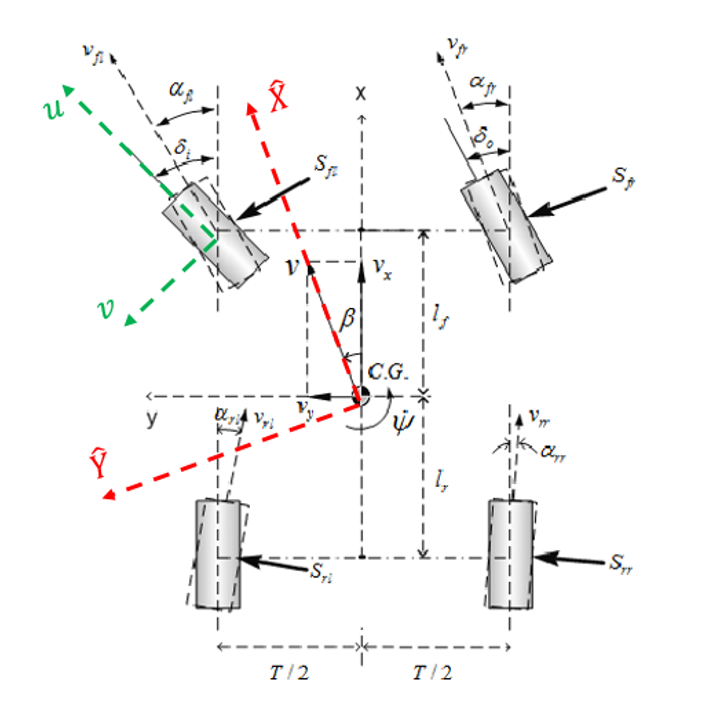
\includegraphics[width=0.7\textwidth]{figures/two-track.png}
    \end{center}
    \caption{Συστήματα αξόνων δίτροχου μοντέλου.}
\label{fig:twotrack_topview}.
\end{figure}


\subsection{Κινηματικές εξισώσεις δίτροχου μοντέλου}

\subsubsection{Εξισώσεις κίνησης οχήματος}

Οι εξισώσεις κίνησης του οχήματος εξάγονται από τις δυναμικές εξισώσεις ισορροπίας των τριών βαθμών ελευθερίας. Οι εξισώσεις κίνησης διατυπώνονται όπως φαίνεται στις \cref{eq:vehicleMotion}

\begin{equation}
  \begin{aligned}
    M\dfrac{d}{dt}U_x(t) &= M\dot{\psi} U_y + F_x\\
    M\dfrac{d}{dt}U_y(t) &= -M\dot{\psi} U_x + F_y\\[10pt]
    I_z\dfrac{d}{dt}\dot{\psi}(t) &=\sum_{i=FL,\dots, RR} \Bigl(\vec{r}_i\times\vec{F}_i\Bigr)_z
  \end{aligned}
  \label{eq:vehicleMotion}
\end{equation}

Όπου:
\begin{itemize}
  \item $M$ η μάζα του οχήματος,
  \item $I_z$ η ροπή αδράνειας του οχήματος γύρω από τον άξονα $z$,
  \item $F_x$ το σύνολο των διαμηκών δυνάμεων των ελαστικών,
  \item $F_y$ το σύνολο των εγκάρσιων δυνάμεων των ελαστικών,
  \item $\vec{F}_i$ το διάνυσμα της δύναμης του ελαστικού $i$,
  \item $\vec{r}_i$ το διάνυσμα θέσης του τροχού $i$ \cref{eq:wheelPositionVectors}.
\end{itemize}

\subsubsection{Υπολογισμός ταχυτήτων των τροχών}

Από το σχήμα \cref{fig:twotrack_topview}, οι ταχύτητα σε κάθε τροχό αποτελεί υπέρθεση της ταχύτητας του οχήματος,
και της εκάστοτε περιφερειακής ταχύτητας λόγω ταχύτητας εκτροπής (\textit{yaw rate}). Στις παρακάτω εξισώσεις οι ταχύτητες
εκφράζονται στο τοπικό σύστημα αξόνων του οχήματος και μετασχηματίζονται αργότερα κατά περίπτωση.

\begin{equation}
  \vec{u}_i = \vec{U}_{CoG} + \vec{\dot{\psi}}\times \vec{r_i}
  \label{eq:wheelVelocity}
\end{equation}

Όπου, ο δείκτης $i$ αναφέρεται σε έναν τροχό (π.χ $i=FL$) και:
\begin{itemize}
\item $\vec{u}_i$ είναι το διάνυσμα της ταχύτητας του τροχού,
\item $\vec{U}_{CoG}$ είναι το διάνυσμα της ταχύτητας του κέντρου μάζας του οχήματος
\item $\vec{r}_i$ είναι το διάνυσμα θέσης 
\end{itemize}

Το διάνυσμα θέσης του κάθε τροχού $\vec{r_i}$ για κάθε τροχό δίνεται από τις εξισώσεις \ref{eq:wheelPositionVectors}.

\begin{equation}
  \begin{aligned}
    \vec{r}_{FL} &= \begin{Bmatrix} a \\ t_f \end{Bmatrix}\\[10pt]
    \vec{r}_{FR} &= \begin{Bmatrix} a \\ -t_f \end{Bmatrix}\\[10pt]
    \vec{r}_{RL} &= \begin{Bmatrix} -b \\ t_r \end{Bmatrix}\\[10pt]
    \vec{r}_{RR} &= \begin{Bmatrix} -b \\ -t_r \end{Bmatrix}
  \end{aligned}
  \label{eq:wheelPositionVectors}
\end{equation}